
\section{Exploring the latent space of StyleGAN}
\label{stylegan}

In this section we will explore very recent\footnote{The InterfaceGan paper was published July this year!} advances in face synthesis and semantic face editing by using a pretrained StyleGan trained by Nvidia.

We can download the weights of a pretrained StyleGan trained by Nvidia directly from their Github.\footnote{\url{https://github.com/NVlabs/stylegan.git}}\cite{stylegan}

This model is trained on the full size and resolution version of the FFHQ dataset.
With the trained generator we can draw samples $z$ from the normal distribution and generate faces $G(x)$ which are near impossible to humans to distinguish from real faces.

In Figure \ref{StyleGAN-examples} we see eight such samples. We can create as many photo realistic faces, of people who have existed, as we want.
\begin{figure}[h!]
  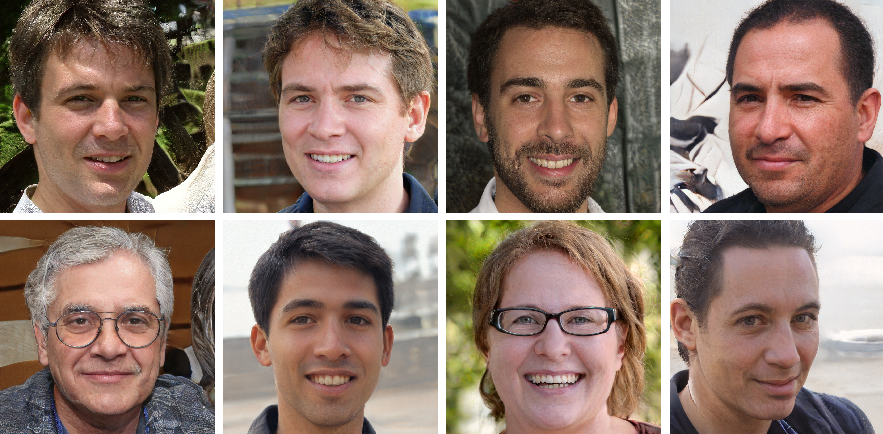
\includegraphics[width=\textwidth]{fig/stylegan/randomsamples}
  \caption{Random samples from the pretrained StyleGAN}
  \label{StyleGAN-examples}
\end{figure}



\subsection{Finding the latent space representation of an arbitrary query image.}

Now the pretrained StyleGAN does not contain an encoder network. Therefore there is no way to find a latent space representation of a arbitrary input image out of the box. This means the even though we can generate an image given a latent representation $z$ there is no way to obtain the latent representation given an arbitrary query image.

The paper \textit{Image2StyleGAN: How to Embed Images Into the StyleGAN Latent Space?}\cite{Image2StyleGAN} explicitly investigates this problem.
In \cite{interfacegan} it is pointed out that there is, a least two different ways of tackling the embedding problem.

\begin{enumerate}
    \item An optimization-based
    approach, which directly optimizes the latent code with fixed generator to minimize the pixel-wise reconstruction error.
    \item An encoder-based approach, where an independent encoder network is trained to learn the inverse mapping.
\end{enumerate}

Here we use a combined apporach \footnote{We use the implementation of a StyleGan encoder available here: \url{https://github.com/Puzer/stylegan-encoder}}
where we first use a ResNet with is trained to directly predict the latent representation in the StyleGan network given an image. The output of the ResNet model is the first approximation of the embedding.

We then proceed to optimize the latent representation using the second apporeach described above. But instead of calculating the loss directly on the pixel-wise reconstruction error we use a pre-trained VGG16 network, where the top part of the network is cut off,  to transform the query image and the reconstructed image into a high dimensional feature space. The loss is then calculated as a difference between the two images in this feature space instead of directly in pixel space. We then iteratively optimize the latent representation to minimize this loss using gradient decent.'

In Figure \ref{stylegan-reconstruction} we see the result of this embedding procedure. In Figure \ref{original} we show the original query images. We choose to embed wikipedia images of Danish politicians. From left to right we see images of Inger Støjberg, Lars Lykke Rasmussen, Mette Frederiken and Uffe Elbæk.

In Figure \ref{firstguess} we see the first approximation given by the ResNet that is trained to output the latent representation given images from StyleGan. We see that although general features like pose and gender is the same as for the original images, the identity of the person in the images generated from this approximation is clearly different.

In Figure \ref{optim} we see the result of optimizing the latent representations for 300 iterations using the VVG16 network, starting from the latent approximation found by the ResNet Network. We see that the result is convincingly close to the original image and we only loose a little bit of the finder details, mainly around the hair region of the images.

\begin{figure}[h!]
    \centering
    \begin{subfigure}[b]{\textwidth}
        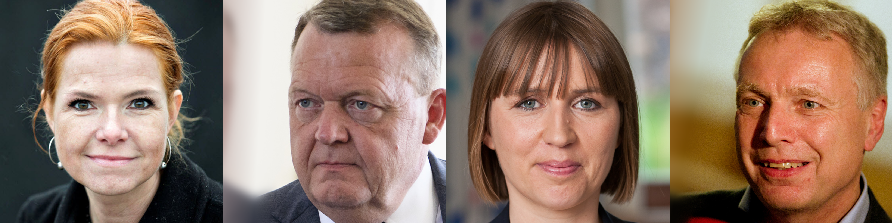
\includegraphics[width=\textwidth]{fig/stylegan/originals}
        \caption{Original images.}
        \label{original}
    \end{subfigure}
    \begin{subfigure}[b]{\textwidth}
    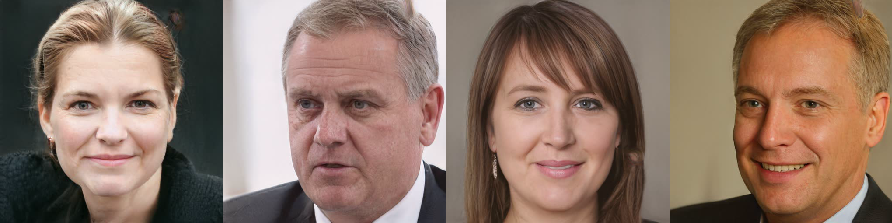
\includegraphics[width=\textwidth]{fig/stylegan/reconstructionsfirstguess.png}
    \caption{First guess of the latent space representation using the pretrained ResNet network}
    \label{firstguess}
    \end{subfigure}
    \begin{subfigure}[b]{\textwidth}
        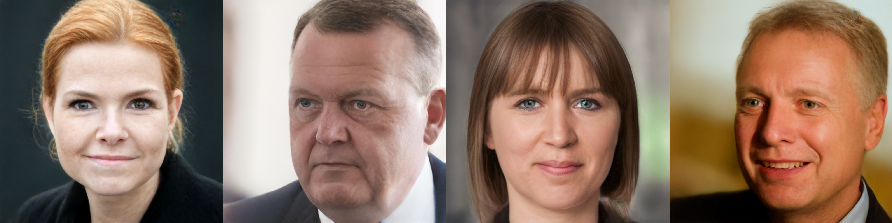
\includegraphics[width=\textwidth]{fig/stylegan/reconstructions}
        \caption{The reconstructed images after optimization using the pretrained VGG16 network.}
        \label{optim}
    \end{subfigure}
    \caption{Comparison of original query images and their reconstruction in the StyleGAN network}
    \label{stylegan-reconstruction}
\end{figure}

We can do a linear interpolation between two latent vectors $z_1$ and $z_2$ simply by
\begin{align}
  z = \alpha z_2 + (1-\alpha)z_1
\end{align}
for $0 \leq \alpha \leq 1$. This linear interpolation results in images that smoothly transitions between faces generated by $z_1$ and $z_2$ respectively. In Figure \ref{StyleGAN-interpolation} we see the result of doing a linear interpolation between the latent representations of the two last danish prime ministers.

\begin{figure}[h!]
  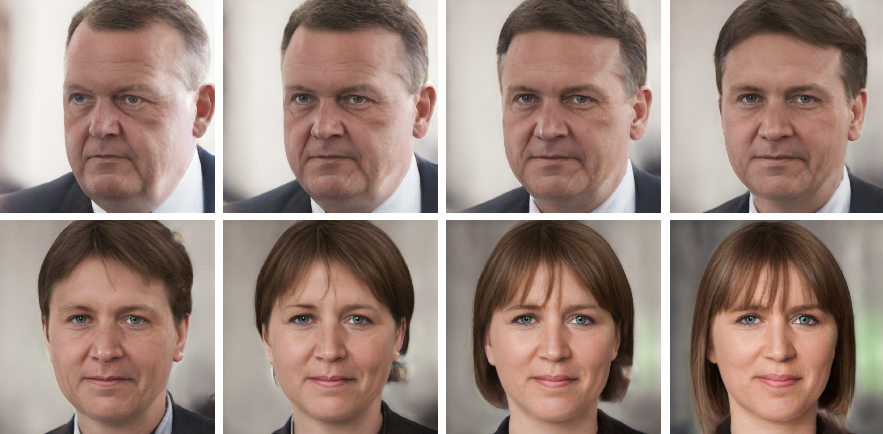
\includegraphics[width=\textwidth]{fig/stylegan/interpolation}
  \caption{Interpolation between two StyleGAN images}
  \label{StyleGAN-interpolation}
\end{figure}




% Optimization is performed only for latent representation which we want to obtain.

% Upon completion of optimization you are able to transform your latent vector as you wish. For example you can find a "smiling direction" in your latent space, move your latent vector in this direction and transform it back to image using the generator.

%
% \begin{figure}[htb]
%     \centering
%     \begin{subfigure}[b]{\textwidth}
%         \centering
%         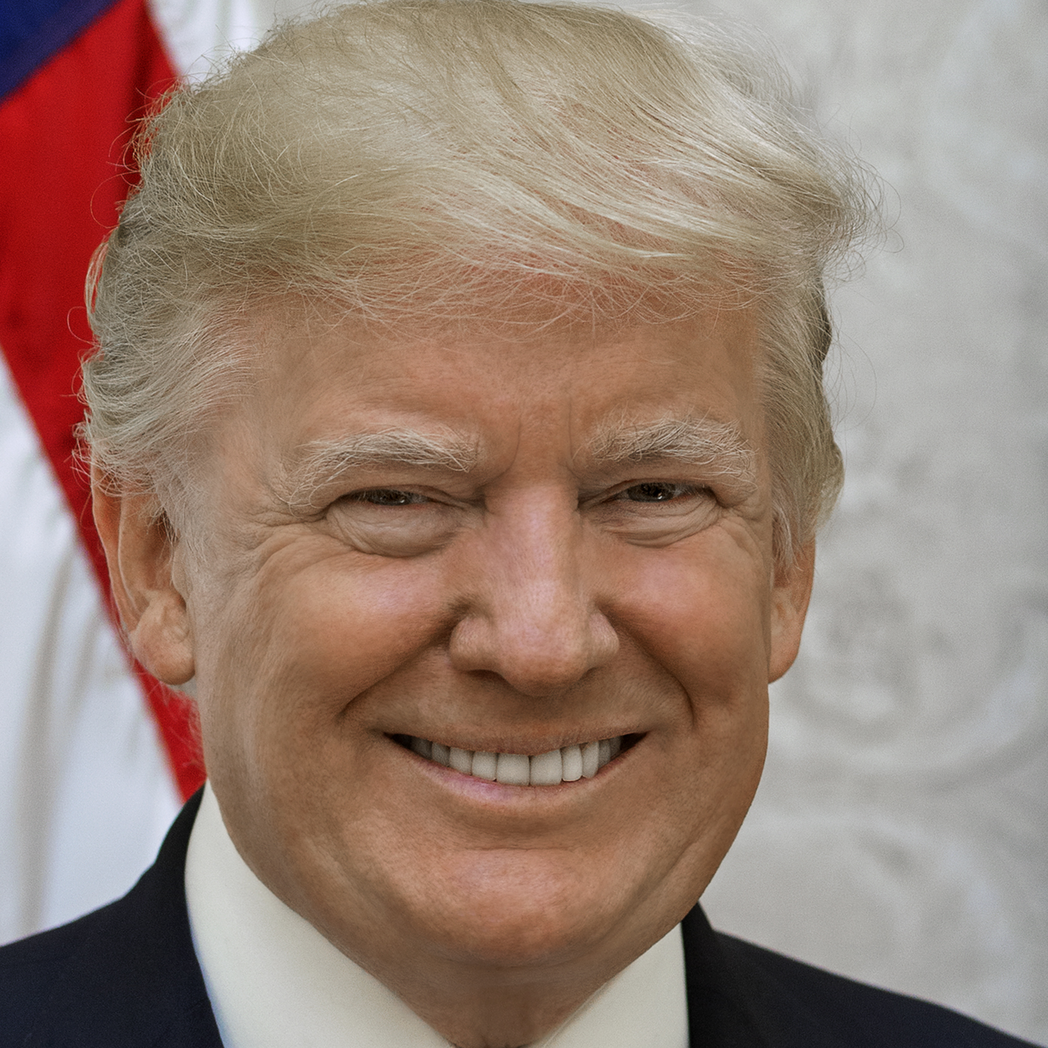
\includegraphics[width=0.3\linewidth]{fig/query_images/trump}%
%         \hfill
%         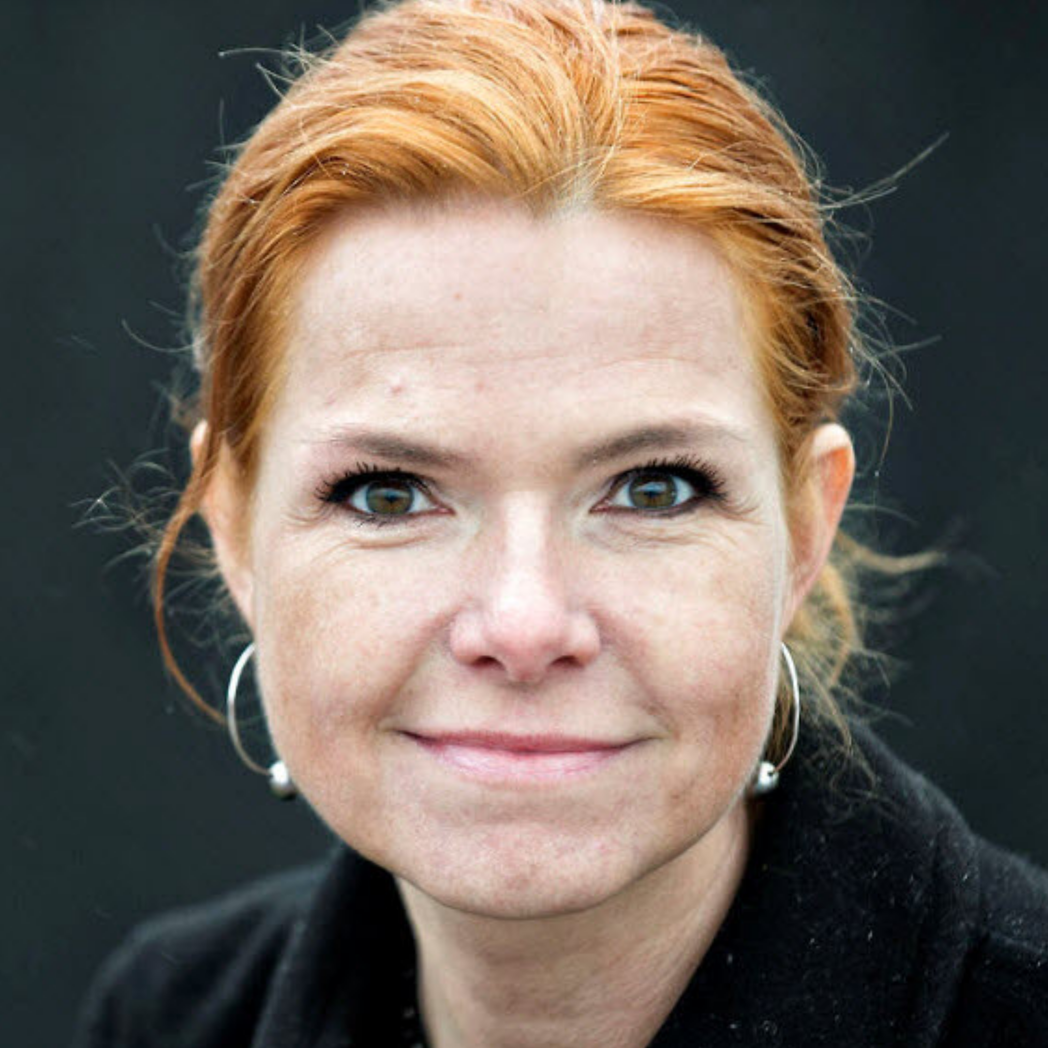
\includegraphics[width=0.3\linewidth]{fig/query_images/inger}
%         \hfill
%         \includegraphics[width=0.3\linewidth]{fig/query_images/skinke}
%         \caption{Original Query Images}
%     \end{subfigure}
%     \vskip\baselineskip
%     \begin{subfigure}[b]{\textwidth}
%         \centering
%         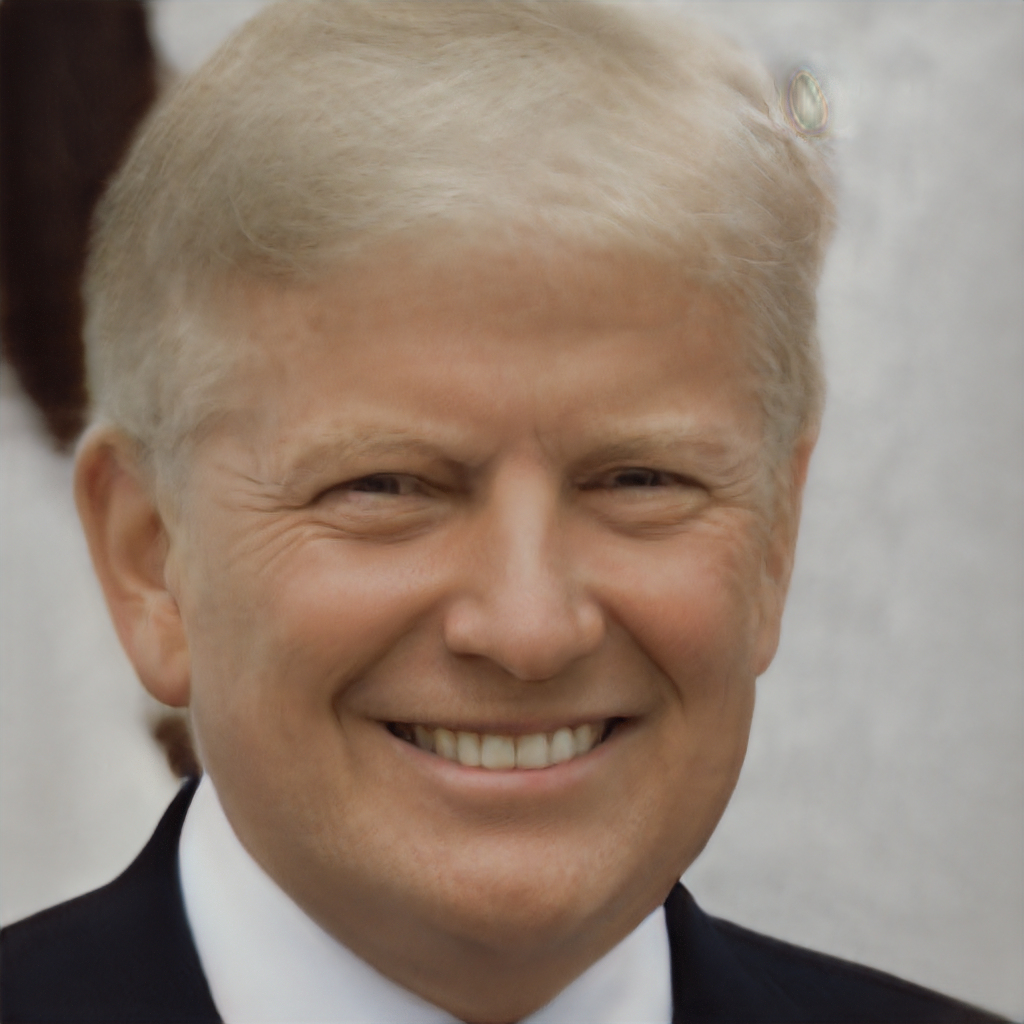
\includegraphics[width=0.3\linewidth]{fig/query_images_reconstucted/trump}%
%         \hfill
%         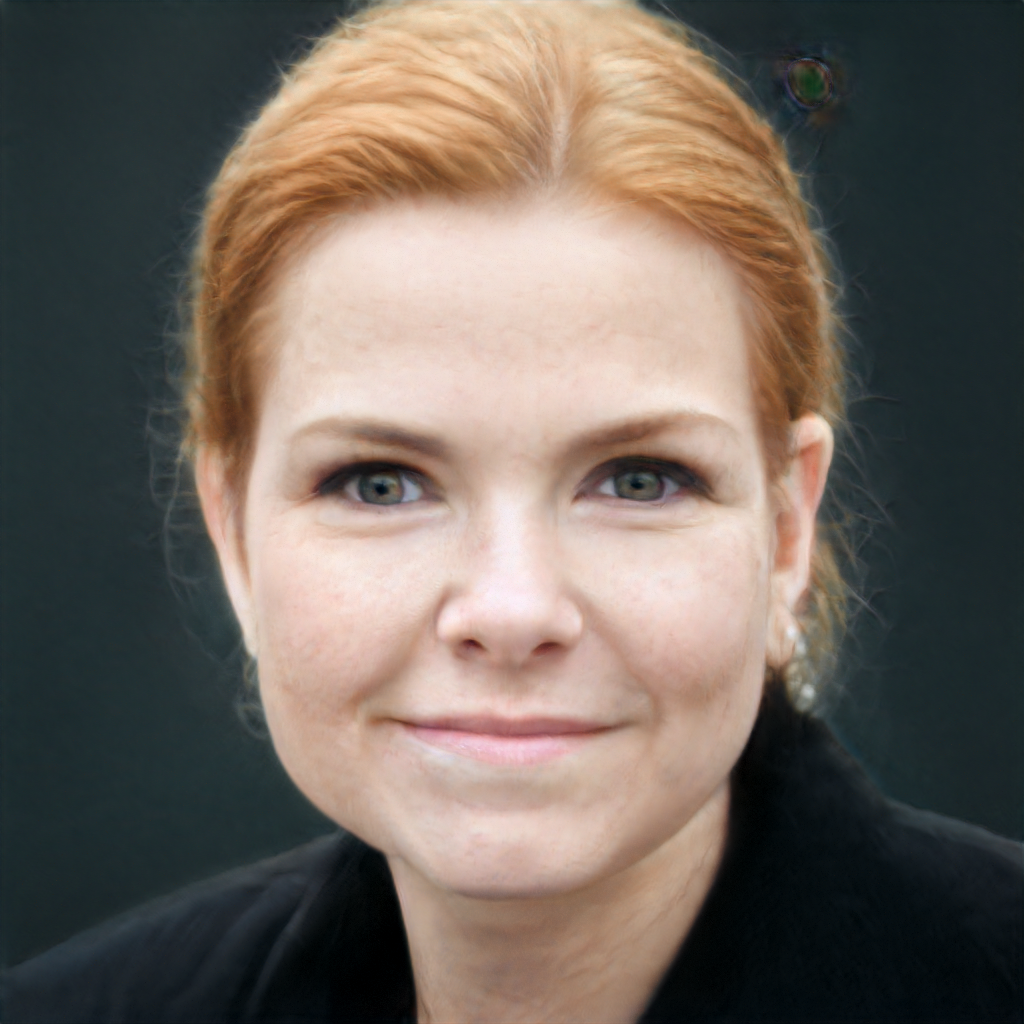
\includegraphics[width=0.3\linewidth]{fig/query_images_reconstucted/inger}
%         \hfill
%         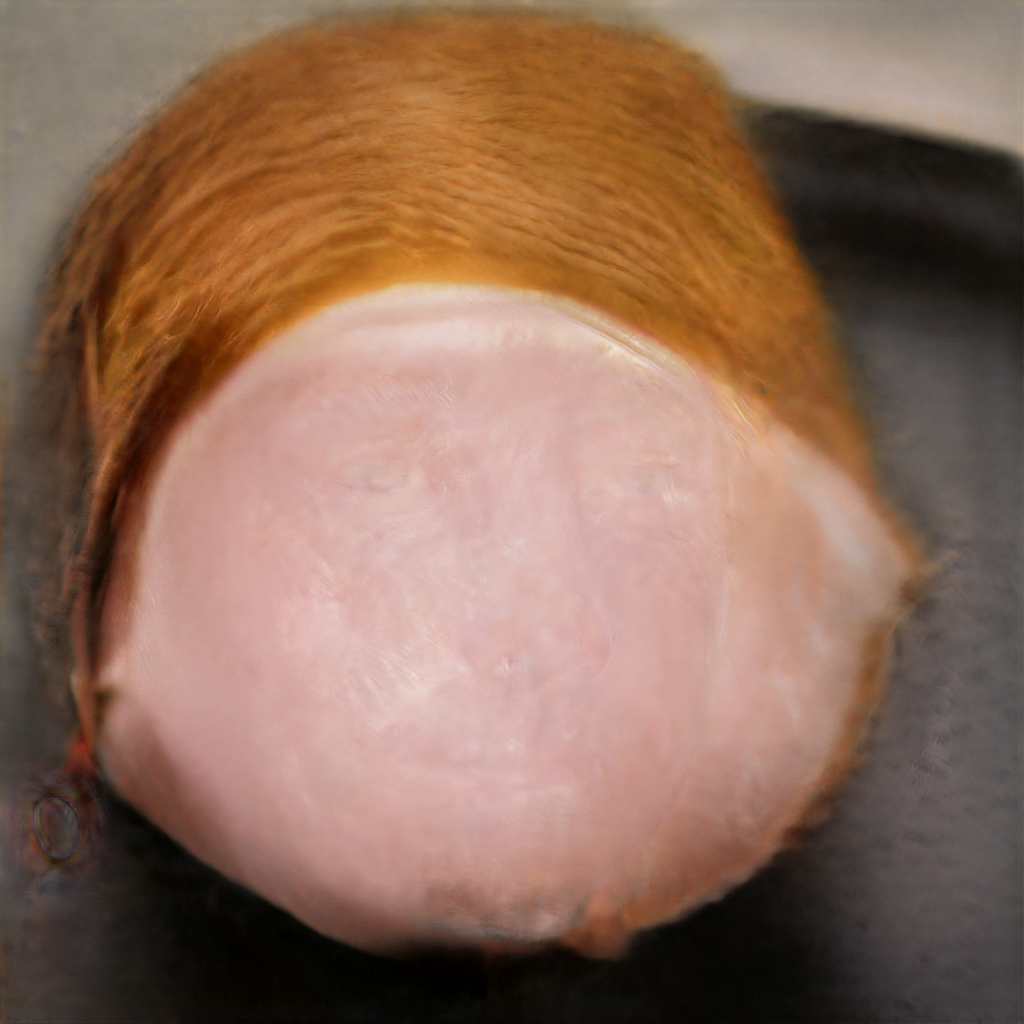
\includegraphics[width=0.3\linewidth]{fig/query_images_reconstucted/skinke}
%         \caption{Reconstructed images from StyleGAN latent space}
%     \end{subfigure}
%     \caption{Latent space representation of arbitrary query images }
% \end{figure}

% \begin{figure}
%     \centering
%     \begin{subfigure}[b]{0.45\textwidth}
%         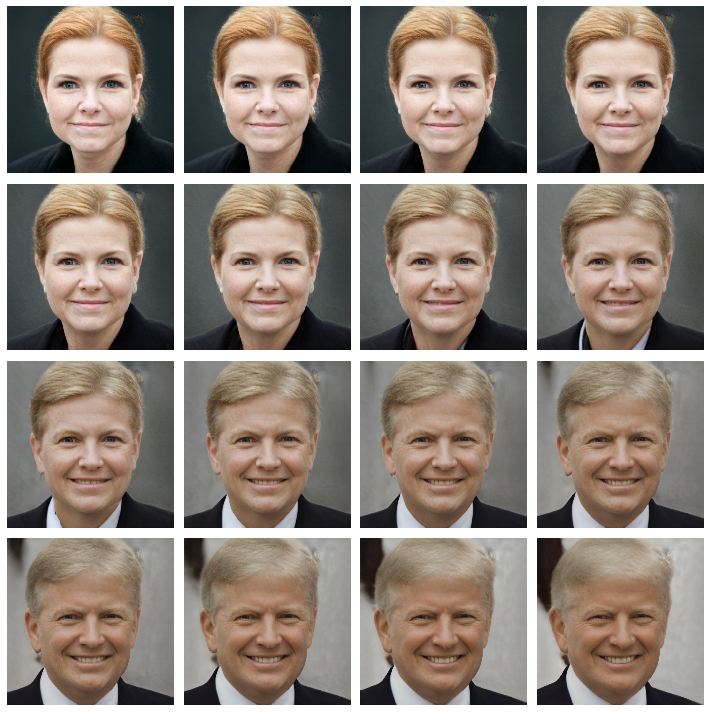
\includegraphics[width=\textwidth]{fig/ingertrump}
%         \caption{Inger Støjberg to Donald Trump}
%     \end{subfigure}
%     ~
%     \begin{subfigure}[b]{0.45\textwidth}
%         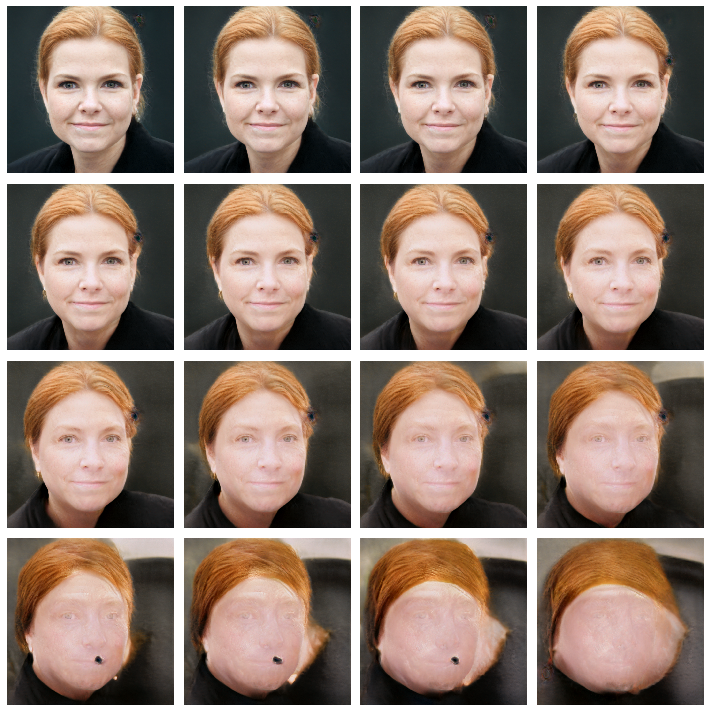
\includegraphics[width=\textwidth]{fig/ingerham}
%         \caption{Inger Støjberg to Ham}
%     \end{subfigure}
%     \caption{Interpolations between query images in the StyleGAN latent space.}
% \end{figure}


To test the robustness of this embedding algorithm we also try and find the latent representation of two query images which are not of faces. Concretely we try to find the latent representation of images of Donald Duck and a ham respectively. We see the results in figure \ref{noface}.

\begin{figure}[h!]
    \centering
    \begin{subfigure}[b]{0.24\textwidth}
        \includegraphics[width=\textwidth]{fig/stylegan/noface/skinke}
    \end{subfigure}
    \begin{subfigure}[b]{0.24\textwidth}
        
\includegraphics[width=\textwidth]{fig/stylegan/noface/and}
    \end{subfigure}

    \begin{subfigure}[b]{0.24\textwidth}
        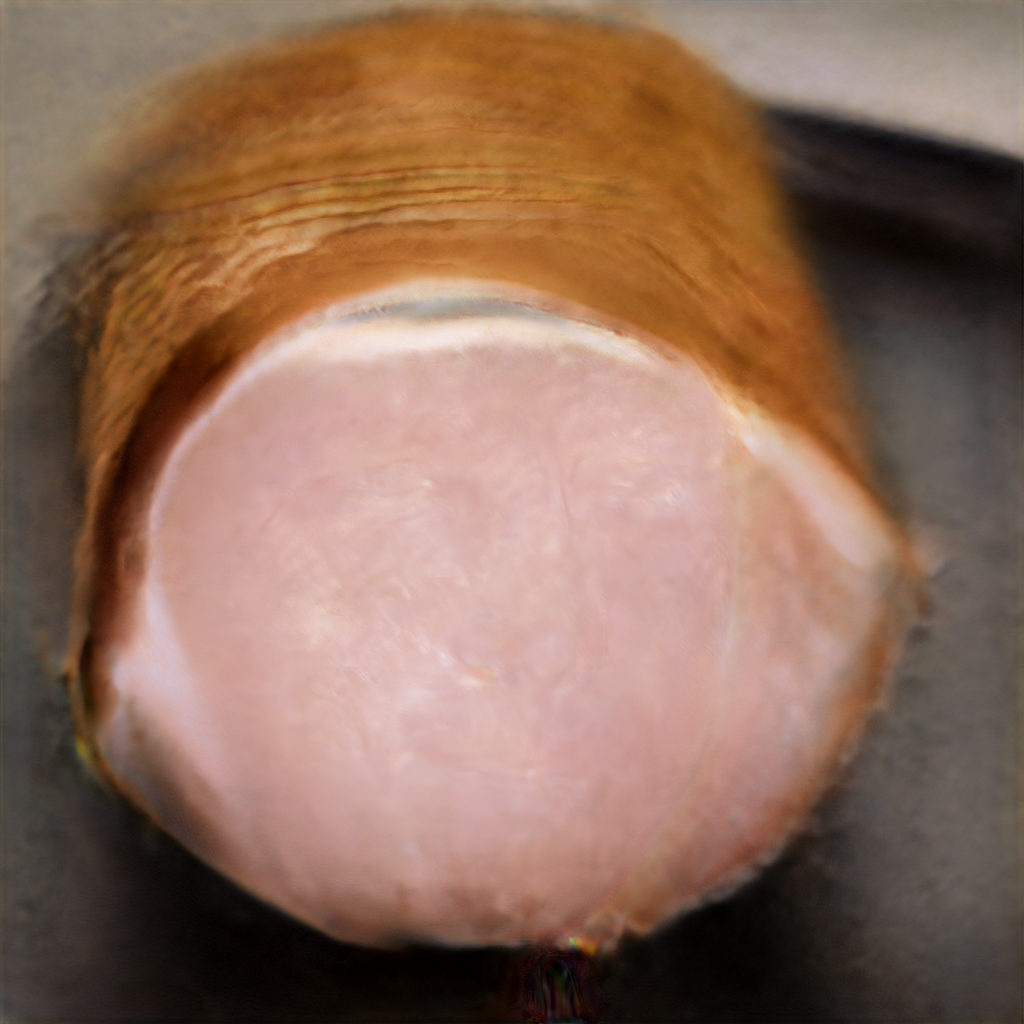
\includegraphics[width=\textwidth]{fig/stylegan/noface/skinkerecon}
    \end{subfigure}
    \begin{subfigure}[b]{0.24\textwidth}
        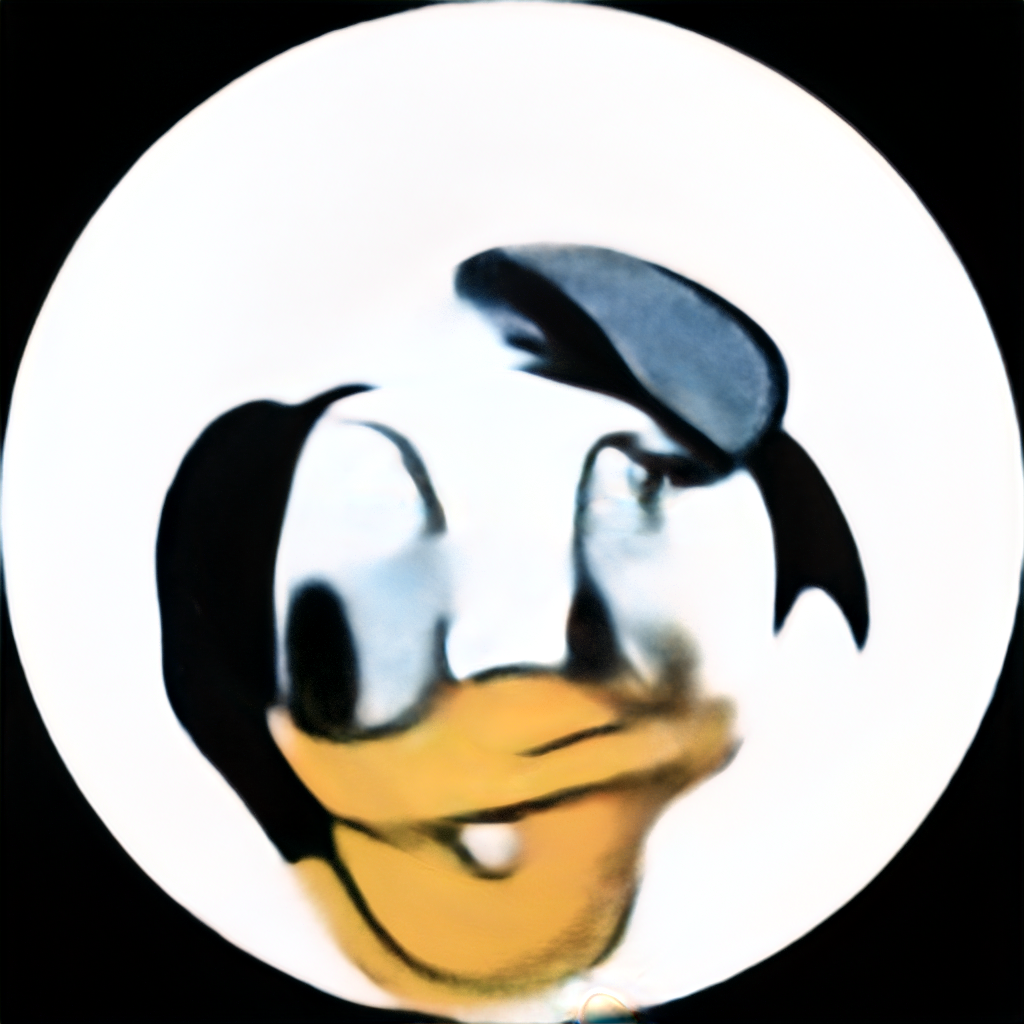
\includegraphics[width=\textwidth]{fig/stylegan/noface/andrecon}
    \end{subfigure}
    \caption{Embedding of query images which are not of faces.}
    \label{noface}
\end{figure}

We see that the reconstruction of the ham is surprisingly good while the reconstruction of Donald Duck is a bit more troubled.

\subsection{Semantic face editing.}
In Figure \ref{faceedit} we see the results from doing semantic face editing of the reconstructed images from \ref{stylegan-reconstruction}. By shifting the latent representations in the direction normal to decision boundaries calculated in \cite{interfacegan} we can edit the images by adding smile, glasses and changing the gender of the respective politicians.

\begin{figure}[h!]
    \centering
    \begin{subfigure}[b]{0.24\textwidth}
        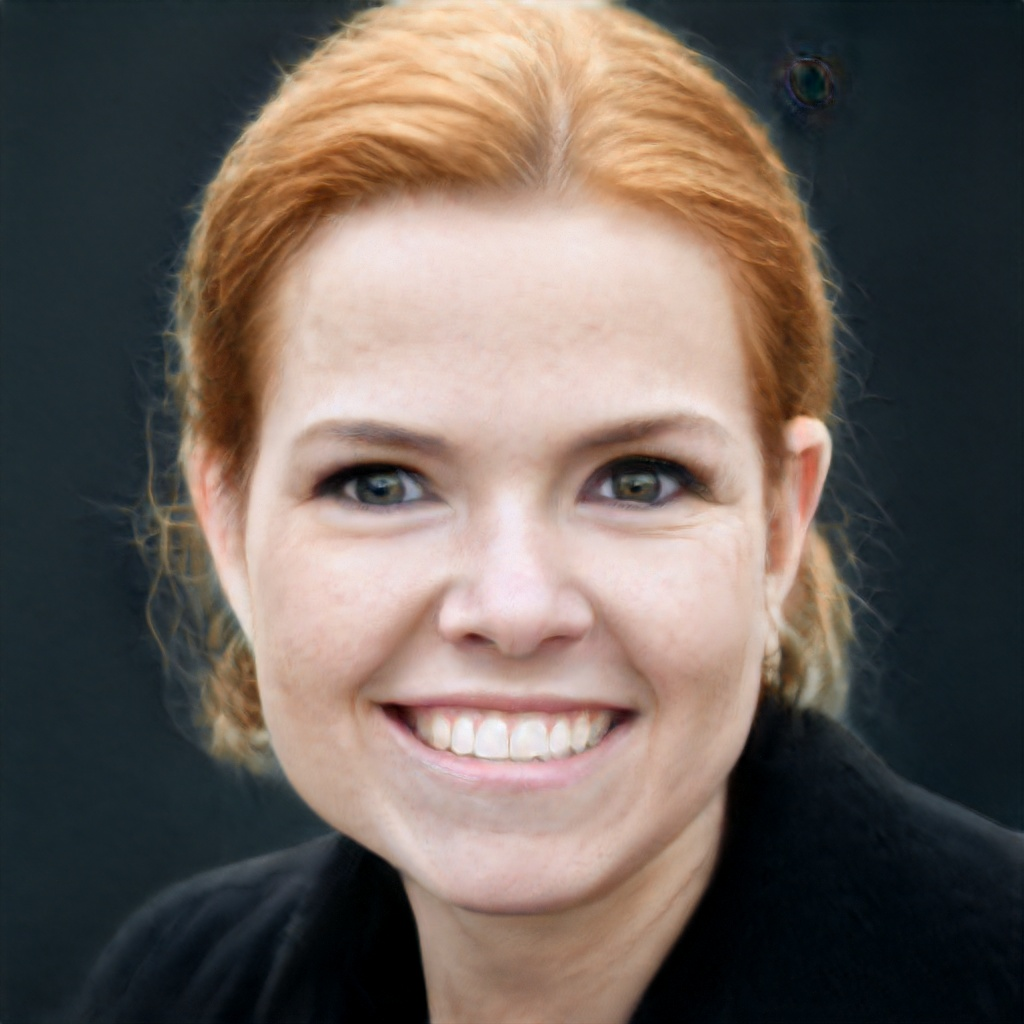
\includegraphics[width=\textwidth]{fig/stylegan/faceedit/inger-smile}
    \end{subfigure}
    \begin{subfigure}[b]{0.24\textwidth}
        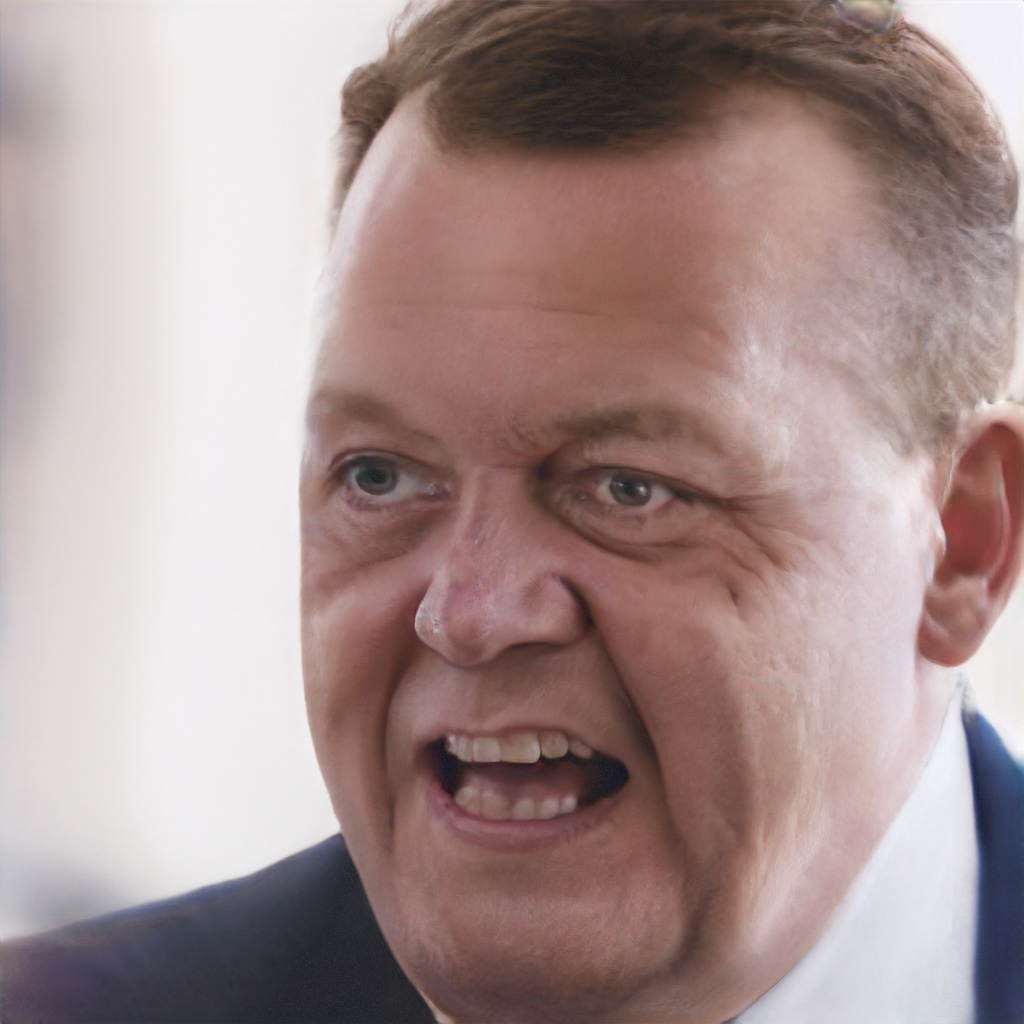
\includegraphics[width=\textwidth]{fig/stylegan/faceedit/lars-smile}
    \end{subfigure}
    \begin{subfigure}[b]{0.24\textwidth}
        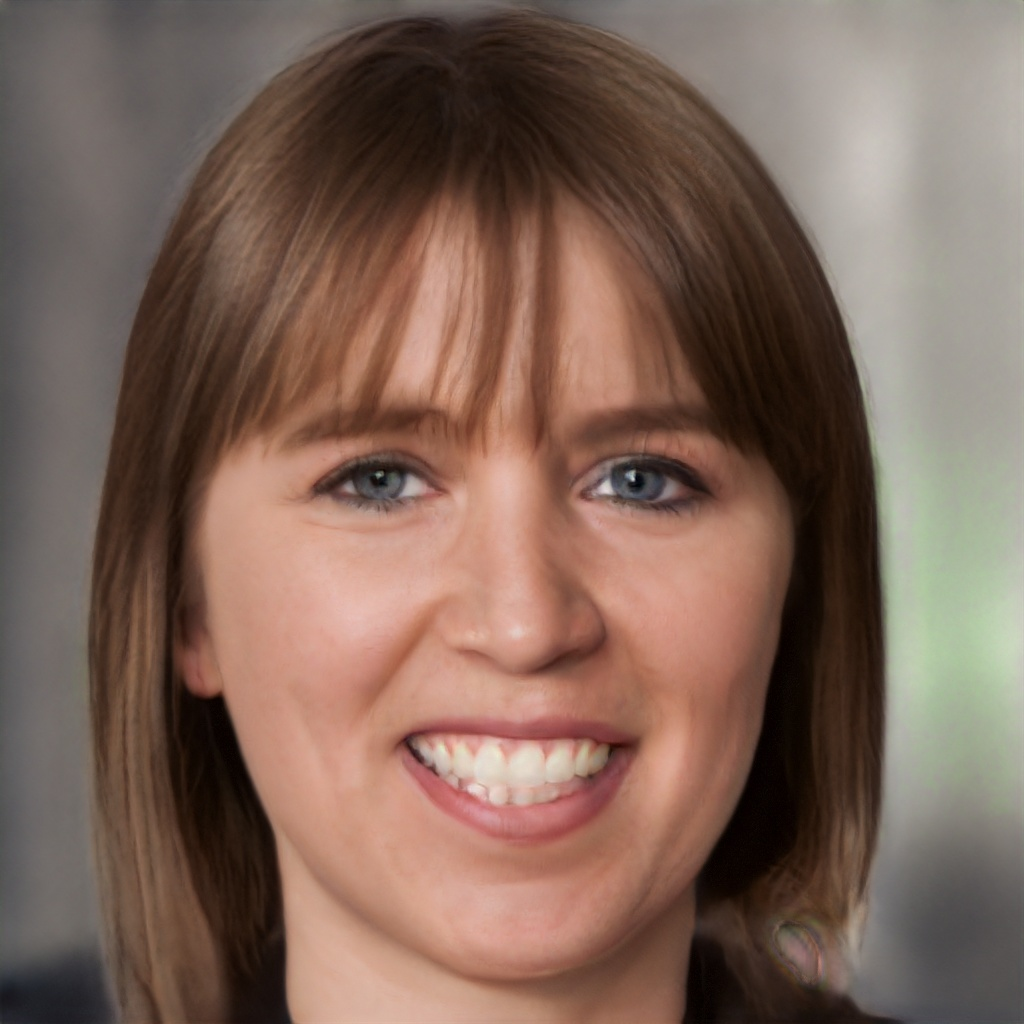
\includegraphics[width=\textwidth]{fig/stylegan/faceedit/mette-smile}
    \end{subfigure}
    \begin{subfigure}[b]{0.24\textwidth}
        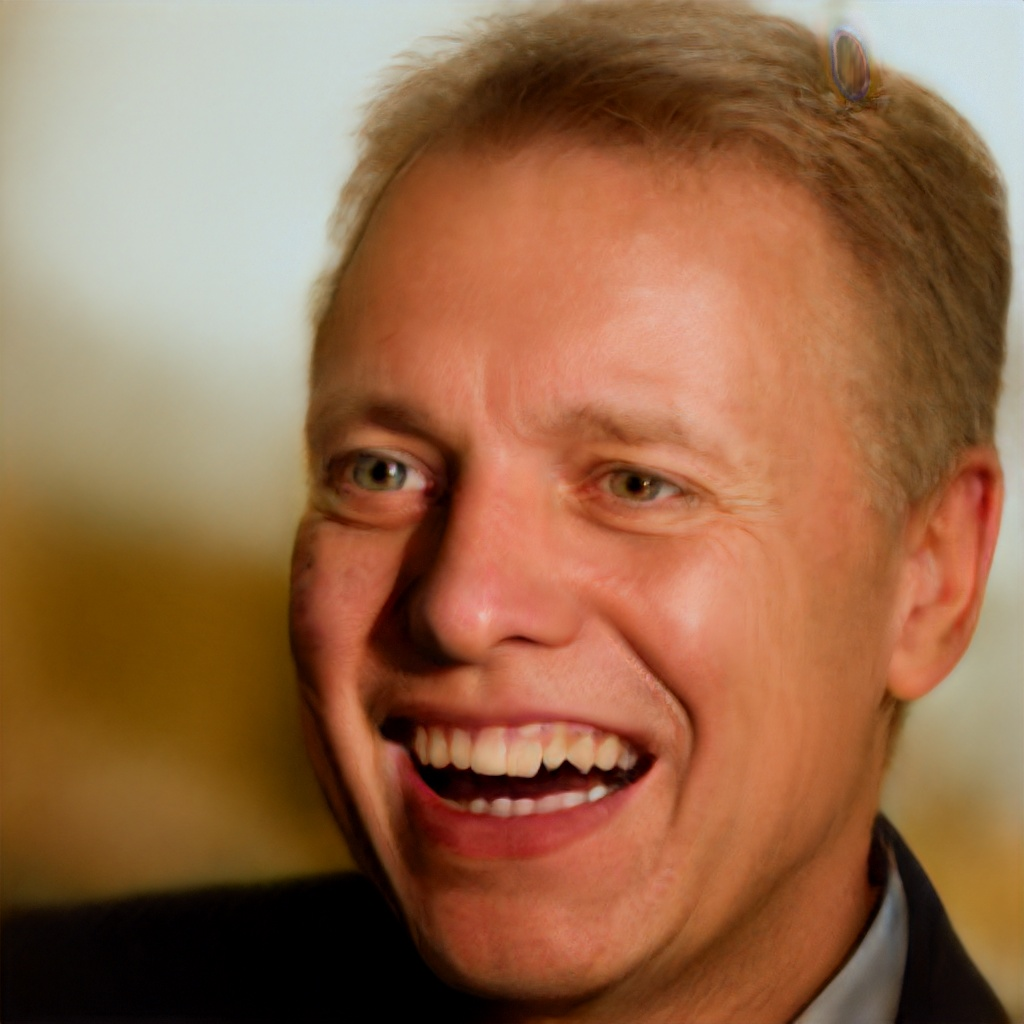
\includegraphics[width=\textwidth]{fig/stylegan/faceedit/uffe-smile}
    \end{subfigure}

    \begin{subfigure}[b]{0.24\textwidth}
        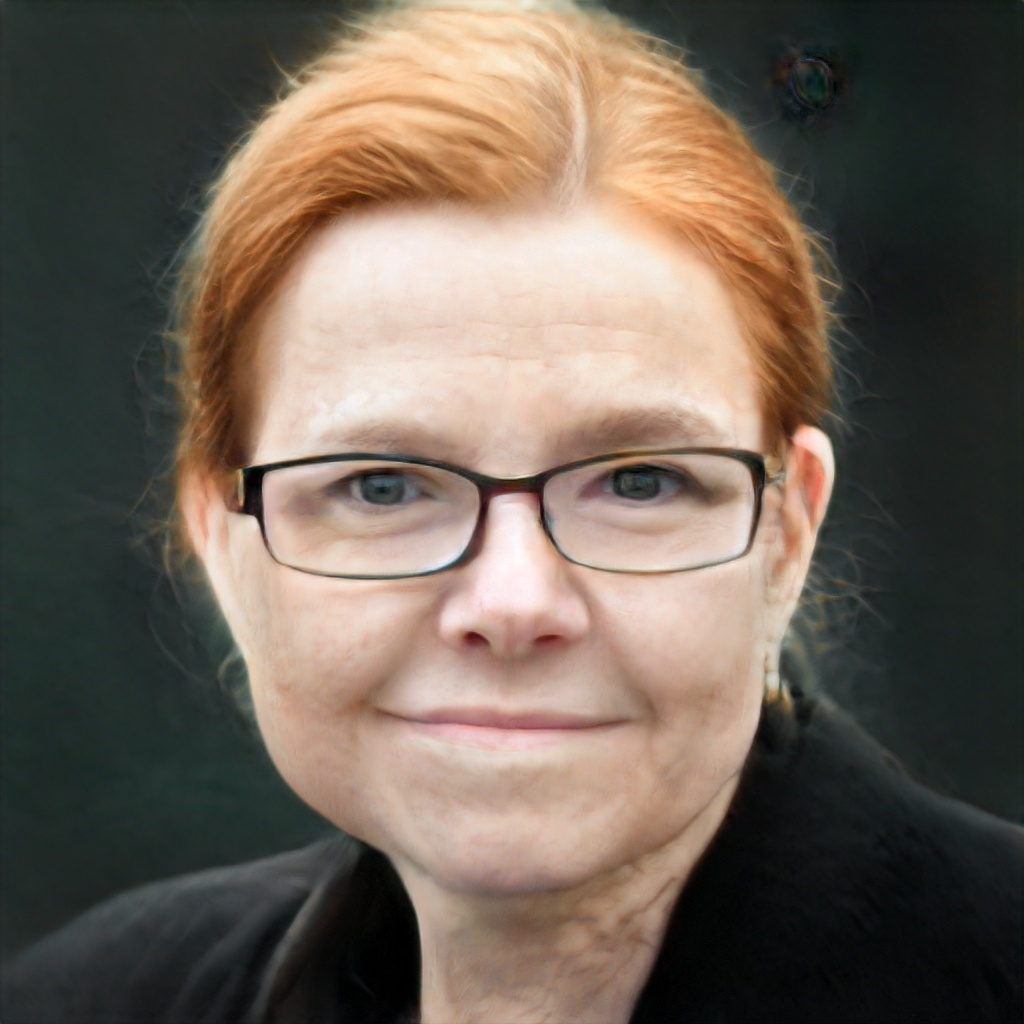
\includegraphics[width=\textwidth]{fig/stylegan/faceedit/inger-glasses}
    \end{subfigure}
    \begin{subfigure}[b]{0.24\textwidth}
        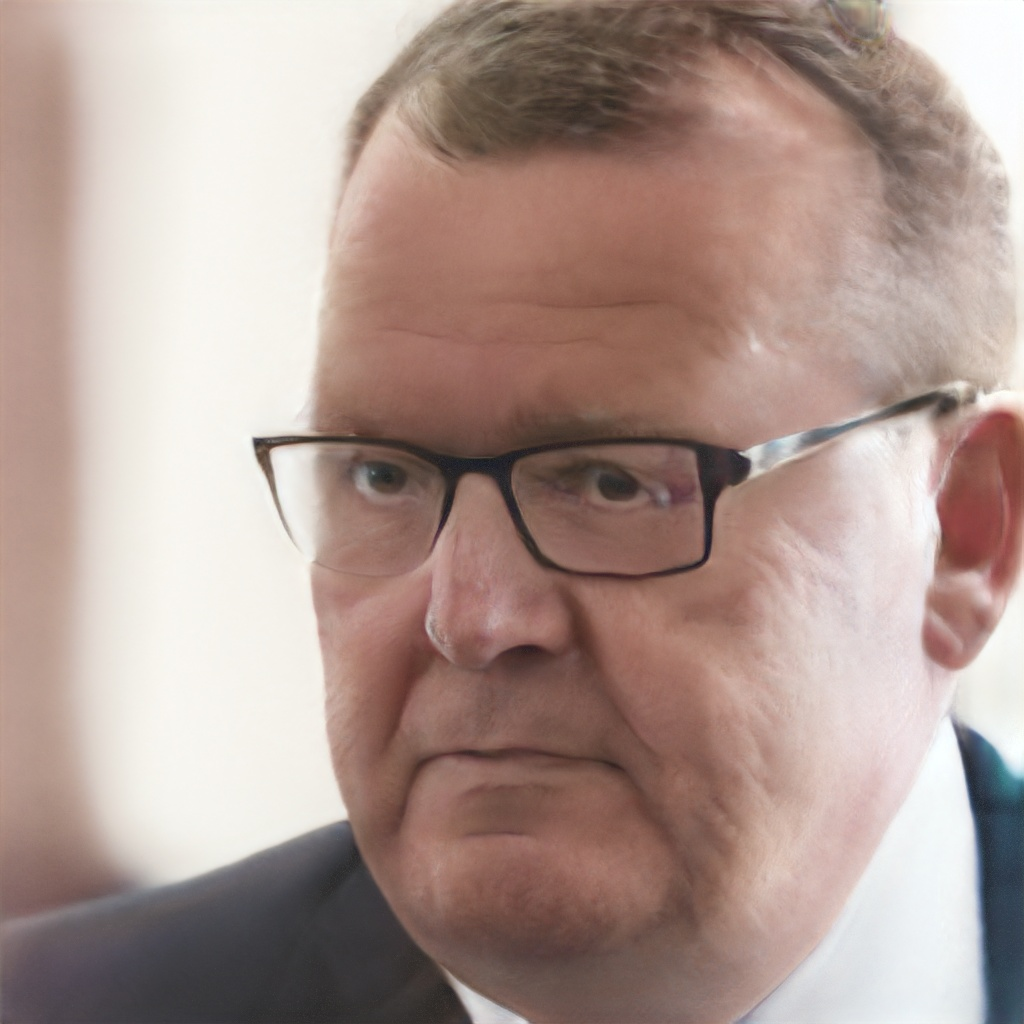
\includegraphics[width=\textwidth]{fig/stylegan/faceedit/lars-glasses}
    \end{subfigure}
    \begin{subfigure}[b]{0.24\textwidth}
        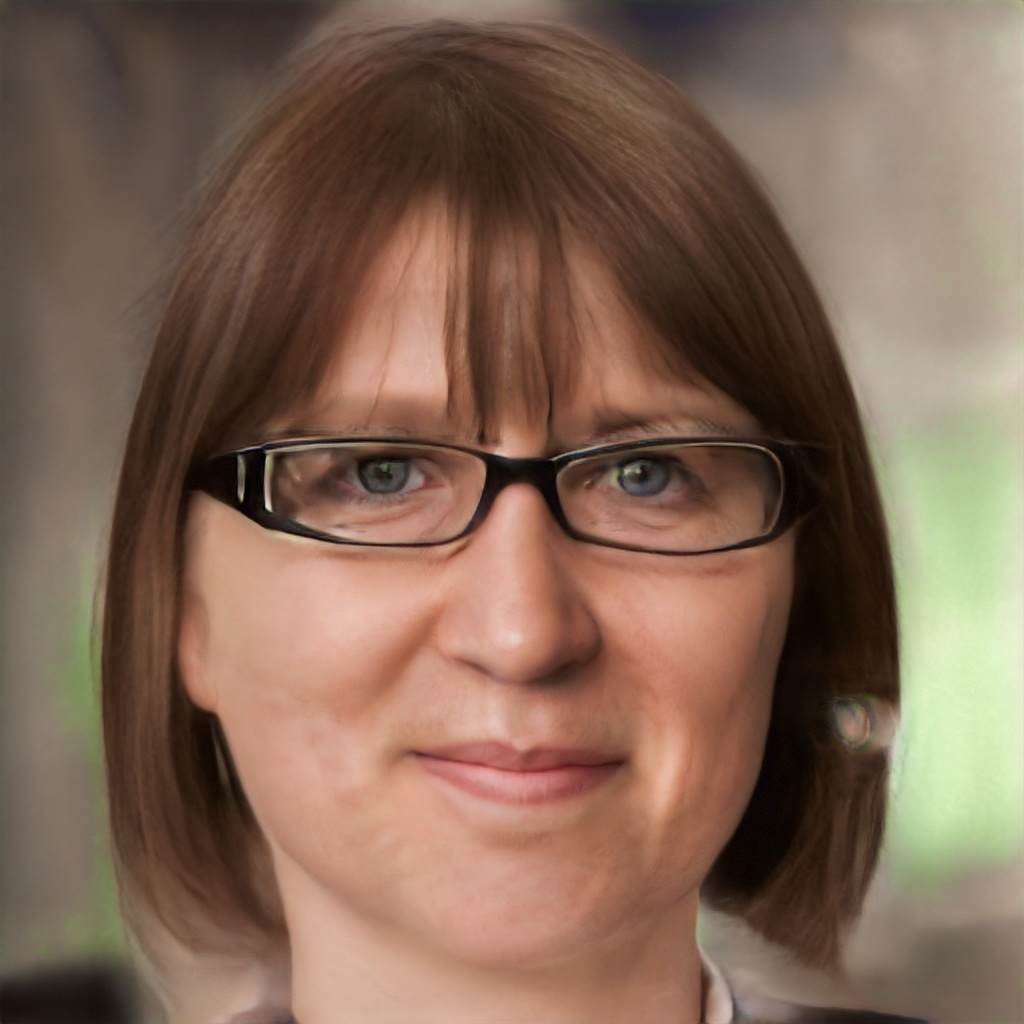
\includegraphics[width=\textwidth]{fig/stylegan/faceedit/mette-glasses}
    \end{subfigure}
    \begin{subfigure}[b]{0.24\textwidth}
        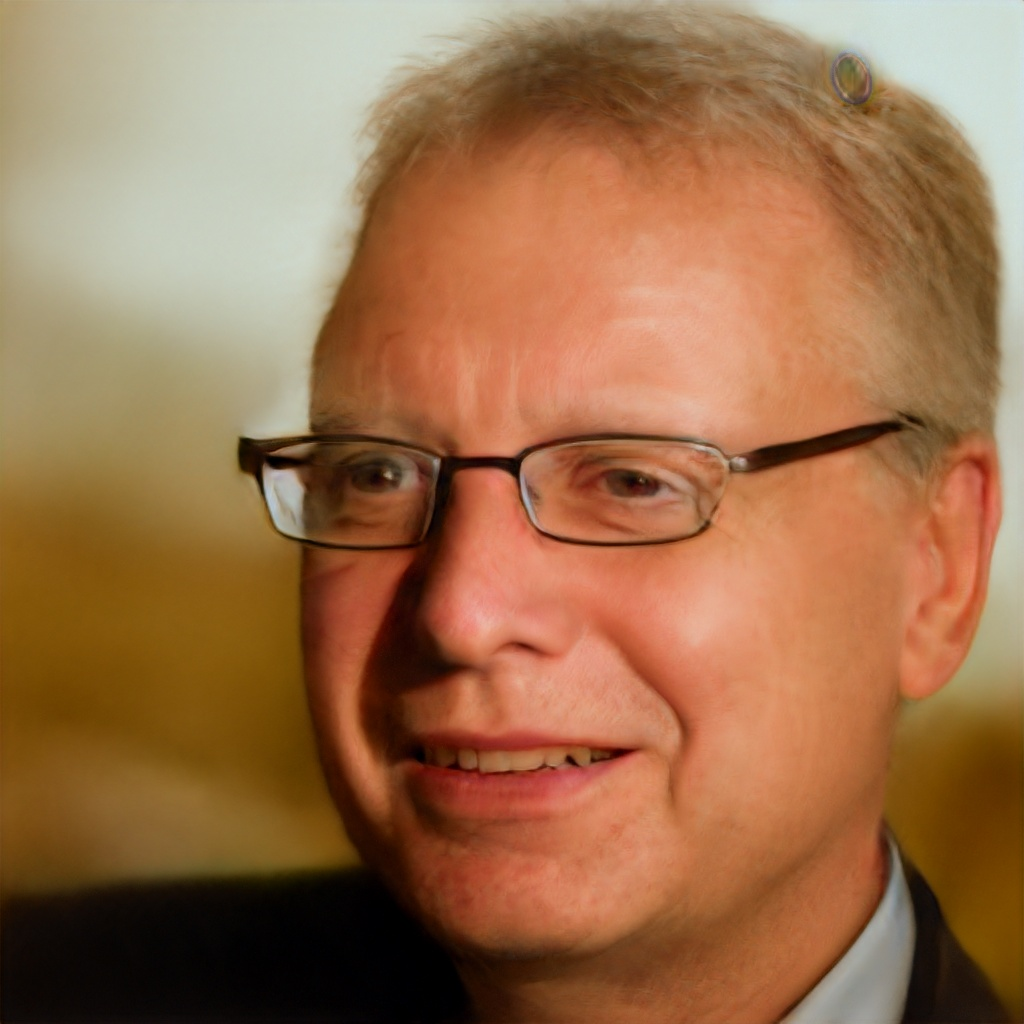
\includegraphics[width=\textwidth]{fig/stylegan/faceedit/uffe-glasses}
    \end{subfigure}

    \begin{subfigure}[b]{0.24\textwidth}
        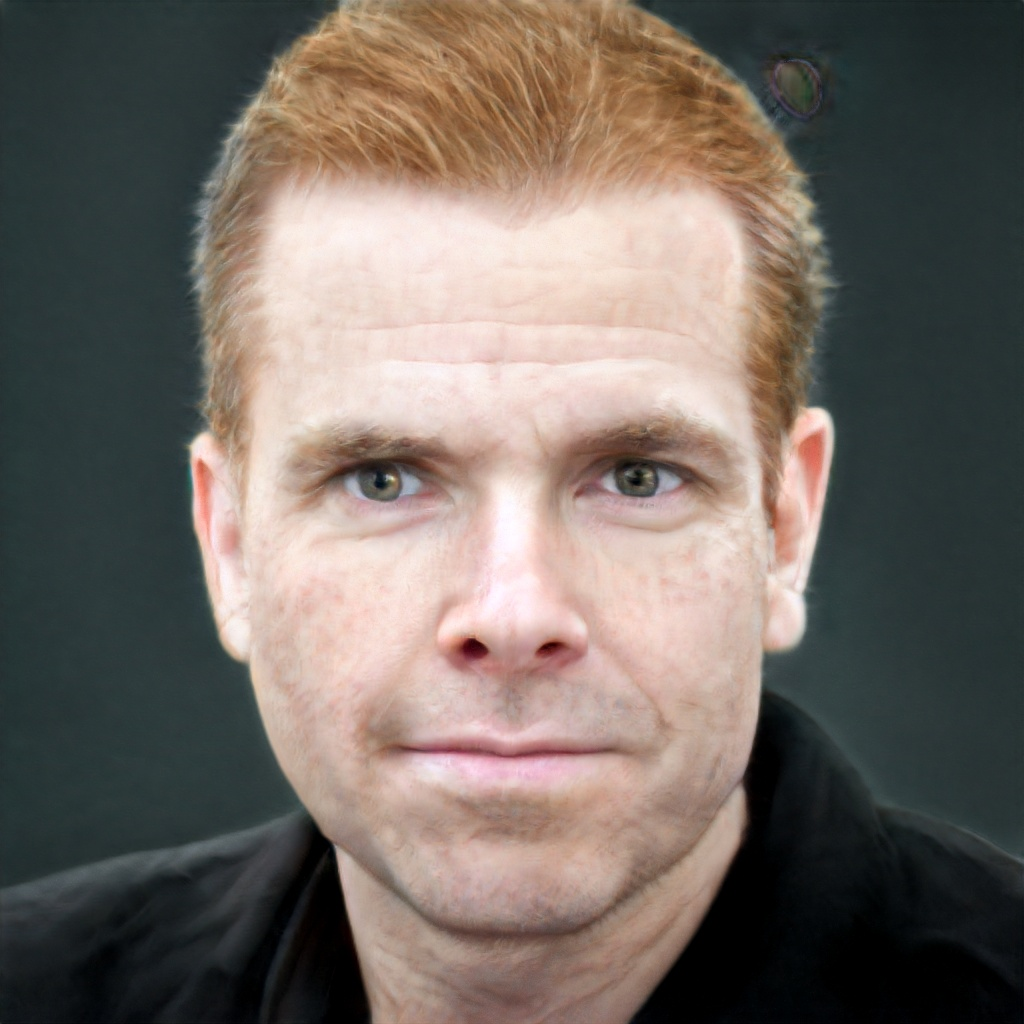
\includegraphics[width=\textwidth]{fig/stylegan/faceedit/inger-gender}
    \end{subfigure}
    \begin{subfigure}[b]{0.24\textwidth}
        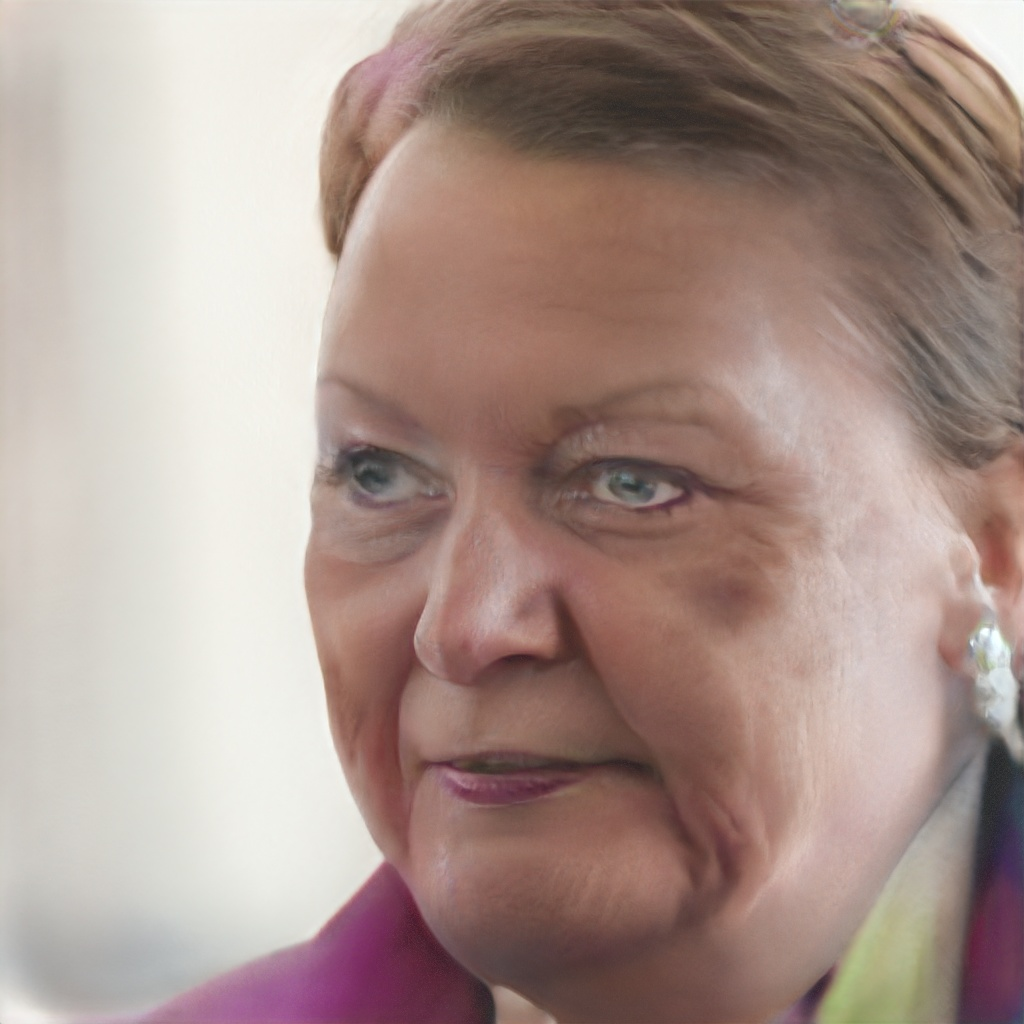
\includegraphics[width=\textwidth]{fig/stylegan/faceedit/lars-gender}
    \end{subfigure}
    \begin{subfigure}[b]{0.24\textwidth}
        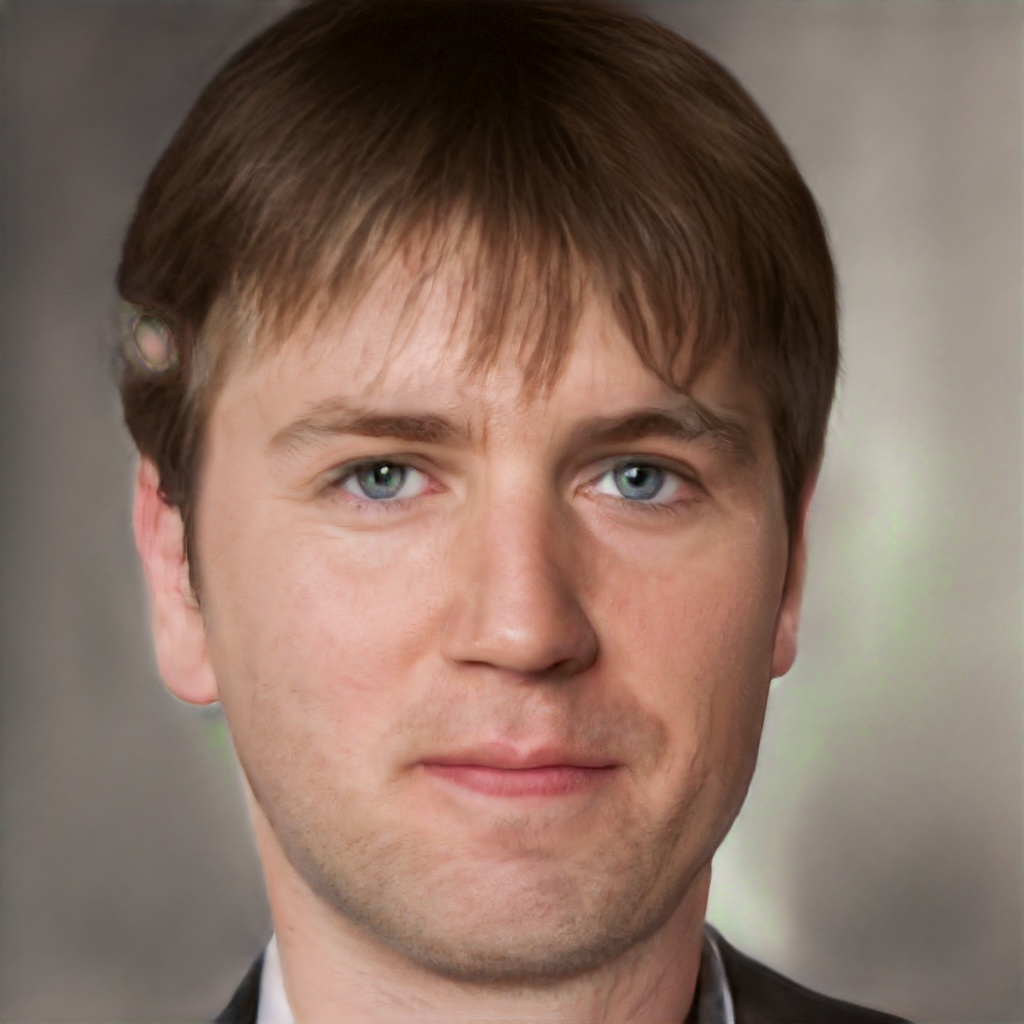
\includegraphics[width=\textwidth]{fig/stylegan/faceedit/mette-gender}
    \end{subfigure}
    \begin{subfigure}[b]{0.24\textwidth}
        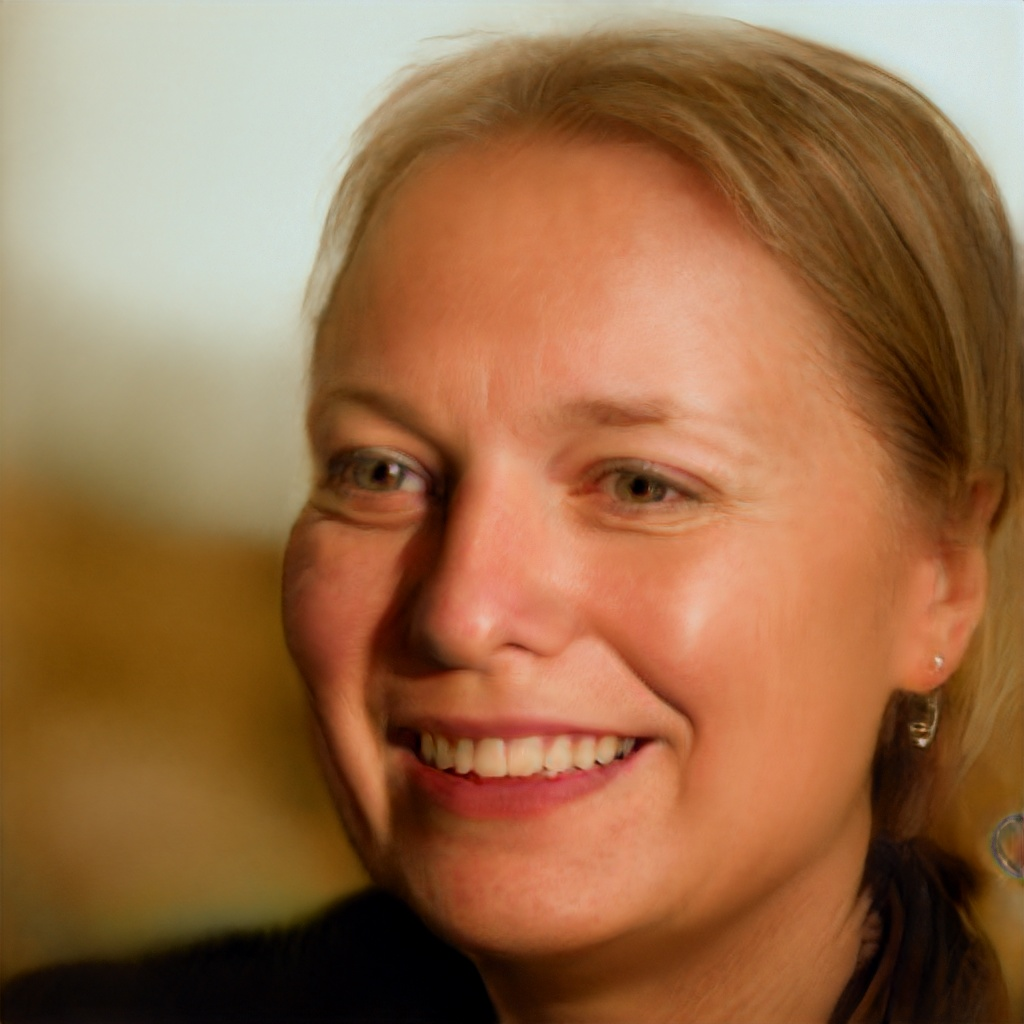
\includegraphics[width=\textwidth]{fig/stylegan/faceedit/uffe-gender}
    \end{subfigure}
    \caption{Semantic face editing. Here we edit the embeddings of Danish politicians by adding smile in the first row, adding glasses in the second row and changing the gender in the third row.}
    \label{faceedit}
\end{figure}
